%=======================================================================
%  Probing and Steering for Safety-Relevant Behaviours in LLMs
%  Draft v3 — 2026-08-02.
%
%  Changes from v2, per review:
%   - v1's title, abstract shape and contributions restored; index terms dropped
%   - framing broadened: the pipeline compares estimators, pooling and layers,
%     not only the read/write dissociation; the UI is a contribution
%   - CAA promoted to a fourth anchor paper; "three papers" phrasing removed
%   - related work back to \paragraph, no per-paper subsections, no "the gap"
%   - method headings follow v1; Detection absorbs the metrics; Implementation
%     and a two-part Evaluation added; divergences woven in rather than sectioned
%   - results restructured per behaviour so each is given its own reading
%   - TikZ diagrams for masking, steering scope, probe grid and the pipeline
%
%  Referencing: HARVARD (author--date) per QMUL Faculty of Science and
%  Engineering. natbib author-year over a manual thebibliography, no .bst needed.
%
%  Build:  latexmk -pdf report_v3.tex
%=======================================================================
\documentclass[conference]{IEEEtran}
\IEEEoverridecommandlockouts

\usepackage[authoryear,round]{natbib}
\usepackage{amsmath,amssymb,amsfonts}
\usepackage{graphicx}
\usepackage{textcomp}
\usepackage{xcolor}
\usepackage{booktabs}
\usepackage{multirow}
\usepackage{url}
\usepackage{float}
\usepackage{tikz}
\usetikzlibrary{positioning,arrows.meta,fit,backgrounds}
\usepackage[hidelinks]{hyperref}

\renewcommand{\bibsection}{\section*{References}}

% Give LaTeX room to place tall full-width floats at page tops rather than deferring
% them to float-only pages (which stranded the steering figure after the Conclusion).
\renewcommand{\topfraction}{0.92}
\renewcommand{\textfraction}{0.06}
\renewcommand{\floatpagefraction}{0.80}
\setcounter{topnumber}{3}
\setcounter{totalnumber}{5}

% Figure slot: renders figures/<file> if present, else a labelled placeholder box.
% Drop the PNGs listed in figures/README.md into figures/ and they appear automatically.
\newcommand{\figslot}[3]{%
  \IfFileExists{figures/#1}%
    {\includegraphics[width=#2]{figures/#1}}%
    {\fbox{\parbox[c][#3][c]{\dimexpr#2-2\fboxsep-2\fboxrule\relax}{\centering
      \textcolor{red}{\scriptsize\texttt{\detokenize{figures/#1}}\\[2pt]not yet captured: see figures/README.md}}}}%
}
\newcommand{\TODO}[1]{\textcolor{red}{[\textbf{TODO:} #1]}}

% Diagram palette
\definecolor{probed}{RGB}{255,236,153}
\definecolor{unprobed}{RGB}{238,238,238}
\definecolor{steered}{RGB}{206,224,255}
\definecolor{readpos}{RGB}{255,205,205}
\definecolor{edge}{RGB}{120,120,120}

\tikzset{
  tok/.style={draw=edge, rounded corners=1pt, inner sep=2pt, font=\scriptsize,
              minimum height=3.6mm, align=center},
  pbox/.style={tok, fill=probed},
  ubox/.style={tok, fill=unprobed},
  sbox/.style={tok, fill=steered},
  rbox/.style={tok, fill=readpos},
  stage/.style={draw=edge, rounded corners=2pt, fill=unprobed, font=\scriptsize,
                align=center, inner sep=3pt, minimum height=6mm},
  fl/.style={-{Latex[length=1.4mm]}, draw=edge},
}

\begin{document}

\title{Probing and Steering for Safety-Relevant Behaviours\\
in Large Language Models}

\author{\IEEEauthorblockN{Nimun Kaur Bajwa}
\IEEEauthorblockA{\textit{MSc Artificial Intelligence}, Queen Mary University of London\\
n.k.bajwa@se25.qmul.ac.uk}}

\maketitle

%=======================================================================
\begin{abstract}
Activation probes are linear readouts used both to \emph{detect} safety-relevant
behaviours and, by adding their direction back into the residual stream, to
\emph{steer} them. These are distinct demands, and prior work has met them
separately: difference-of-means directions are reported as the most causally
implicated, logistic-regression probes as the best detectors. Read together this
suggests a \emph{read/write dissociation}, in which the direction that best reads
a behaviour is not the one that best writes it. No prior work tests this
within a single pipeline, and the suggestion could equally be an artefact of the
differing models, metrics and token policies involved. We build such a pipeline,
fixing estimator, pooling, layer and intervention site uniformly, and apply it to
deception, high-stakes awareness and sycophancy in Llama-3.1-8B-Instruct. The
dissociation replicates on the first two, where logistic regression wins 75\% and
100\% of detection comparisons and mass-mean wins every steering comparison. It
\emph{inverts} on sycophancy, where mass-mean is simultaneously the best
out-of-distribution detector and among the worst steerers. Scoring steered
generations for coherence as well as behaviour supplies a partial explanation the
causal metric alone cannot. Mass-mean degrades generation quality at high
strengths where other directions do not, so part of its causal advantage is
steering harder rather than better. The dissociation is therefore a property of
particular behaviour--representation pairs, not a general law.
\end{abstract}

%=======================================================================
\section{Introduction}

As language models are deployed in consequential settings, cheap monitoring of
their internal state becomes a practical safety requirement. \emph{Activation
probes}, linear readouts of the residual stream, are a leading candidate,
flagging a property of interest at a fraction of the cost of an auxiliary monitor
model \citep{alain2018,mckenzie2025}. Two questions decide whether such a probe is
useful: does it \emph{detect} the property, separating positives from negatives
both in- and out-of-distribution; and is the direction it finds
\emph{causally implicated}, such that adding it to the residual stream changes
what the model does?

The second question is a necessary control rather than a curiosity, and
\citet{marks2024} are explicit about why. Reviewing the failure of earlier truth
probes to generalise to statements containing ``not'' \citep{levinstein2024}, they
observe that such results suggest ``these probes may be identifying \emph{not}
truth, but other features that \emph{correlate} with truth on their training
data.'' A probe can therefore score a high AUROC while reading a confound.
Testing whether \emph{writing} the direction back in changes the output
distinguishes a direction the model uses from one that merely co-varies with the
label. Detection performance alone cannot establish that a probe found the
behaviour.

Prior work answers these two questions separately and on different properties.
\citet{marks2024} find that difference-of-means (``mass-mean'') directions for
truth are the most causally implicated, beating logistic regression in 7 of 8
intervention conditions \emph{despite} comparable classification accuracy.
\citet{goldowsky2025} (Apollo) find logistic-regression probes the strongest
detectors of strategic deception. \citet{mckenzie2025} find that probes pooling
over the whole sequence detect high-stakes interactions far better than
last-token probes. \citet{rimsky2024} show that mean-difference directions steer
open-ended generation when added during decoding, graded by an LLM judge.

Together these suggest a \emph{read/write dissociation}: the direction that best
reads a behaviour may not be the one that best writes it. But the suggestion is
fragile. The results come from different models, behaviours, metrics and token
policies, so any apparent dissociation could be an artefact of that heterogeneity.
Testing it requires holding everything else fixed, which in turn requires settling
questions the individual papers answer differently: which estimator to fit, which
tokens to pool, which layer to read from, and where to intervene. These choices are
not incidental. At least one of them turns out to matter more than the estimator.

\subsection*{Contributions}
\begin{itemize}
  \item \textbf{The first test of the read/write dissociation on safety
  behaviours}: for each behaviour the same activations yield mass-mean,
  logistic-regression and attention probes for detection and for steering, under
  one protocol, so ``which detects best'' and ``which steers best'' are directly
  comparable.
  \item \textbf{A uniform comparison of the choices the question depends on}:
  estimator, token pooling and layer are varied within one pipeline rather than
  across papers, which surfaces a case where pooling matters more than the
  estimator.
  \item \textbf{A layer-selection method for behaviours lacking a token-level
  readout}: a normalised-indirect-effect sweep with a baseline-separability gate,
  standing in for the interchange-patching localisation of \citet{marks2024} where
  a one-token minimal pair is unavailable.
  \item \textbf{A reusable pipeline}: each behaviour is one specification (data,
  masking, readout, steering mode) run through identical machinery, so behaviours
  are comparable and new ones are added as configuration. Deception, high-stakes
  awareness and sycophancy here; user intention, refusal and sparse-autoencoder
  latents planned.
  \item \textbf{An interactive interface} over the exported probes and directions:
  a user can score their own text with any probe in the grid and steer generation
  at a chosen coefficient, making the artefacts inspectable rather than only
  tabulated.
\end{itemize}

Our code, datasets, and the interface are available at
\url{https://github.com/NimunB/probing-safety-behaviours}.

%=======================================================================
\section{Related Work}

\paragraph{Linear representations and probing}
That models represent features as directions in activation space, so a linear
readout can recover them, is the premise here \citep{alain2018,elhage2022}.
Probing for truthfulness was advanced by \citet{azaria2023} and by
\citet{burns2023}, whose Contrast-Consistent Search finds a truth direction
without labels. \citet{levinstein2024} then showed such probes fail to generalise
in basic ways, suggesting they track correlates of truth rather than truth itself.
For that reason we treat out-of-distribution evaluation as the only informative
column below, and include causal testing at all.

\paragraph{Causality, and mass-mean probing}
\citet{marks2024} answer that critique with curated true/false datasets built to
minimise non-truth variation, and supply three things used directly here. They
localise representations by \emph{activation patching}, swapping residual-stream
activations at each (position, layer) between a minimal prompt pair, isolating a
small group of causally implicated states over the statement-end tokens. They
introduce mass-mean probing, $\boldsymbol{\theta}_{\mathrm{mm}} =
\boldsymbol{\mu}^{+} - \boldsymbol{\mu}^{-}$, with a covariance-corrected variant
for in-distribution use. And they quantify causality with a \emph{normalised
indirect effect} (NIE): the shift a direction induces in the model's own TRUE/FALSE
readout, in units of the unsteered class gap. Their finding that mass-mean is most
causal despite comparable accuracy is the asymmetry this work generalises.
Inference-time intervention \citep{li2023} and causal mediation
\citep{vig2020,meng2022} give the broader framing of directions as mediators.

\paragraph{Detection: estimators, pooling and metrics}
Apollo \citep{goldowsky2025} train on \emph{instructed pairs} --- the same fact
under honest and dishonest system prompts, so the activation difference encodes
intent and the training set contains no actual deception. Their probe is fitted
per-token and scored by averaging per-token projections over the response, on
evaluation sets including AI Liar \citep{pacchiardi2024} and insider trading
\citep{scheurer2023}, with false positives calibrated against unrelated
instruction-following responses \citep{taori2023}. Their appendix finds
difference-of-means, LDA and logistic regression ``very similar'' at separating
honest from deceptive responses, with logistic regression winning only on
separating deception from \emph{unrelated} text. \citet{mckenzie2025} contribute
the pooling axis: comparing mean, max, last-token, softmax- and
attention-weighted aggregation, they find learned pooling superior (following
\citealt{kantamneni2025}), and select their layer by cross-validation on the
training set, the protocol adopted below.

\paragraph{Steering, and judging its effect}
CAA \citep{rimsky2024} builds steering vectors as mean activation differences over
contrast pairs, adds them during decoding with a signed multiplier, and scores
generations 1--10 with an LLM judge. Two details shape the design here: it steers
only \emph{generated} tokens, leaving the prompt untouched, and it derives its
open-ended prompts from the same held-out items as its constrained evaluation,
which is what keeps seven behaviours comparable. It also reports that large
multipliers degrade text quality and responds by restricting the range. This work
measures quality explicitly instead.

\paragraph{Sycophancy}
Deferring to a user's stated belief over an accurate answer is documented as an
artefact of preference-based training \citep{perez2023,sharma2023}. The factorial
datasets of \citet{cincynlp2025} supply a \emph{genuine-agreement} control, in which
the user happens to be correct so that agreement is candid. This makes sycophancy a
discriminating third case rather than a repetition of the first two.

%=======================================================================
\section{Method}

Because the comparison rather than the absolute performance is the deliverable,
the design is driven by a small set of requirements, each of which forces a
choice later in this section.

\textbf{R1: Matched arms.} Every estimator must be compared under identical
conditions: same layer, same tokens, same calibration, same intervention site.
Any asymmetry becomes a confound.

\textbf{R2: Both sides need a metric, and each must be fixed before the
comparison.} On the read side the anchor papers disagree: accuracy
\citep{marks2024}, AUROC with recall at 1\% FPR \citep{goldowsky2025}, AUROC
\citep{mckenzie2025} --- so one choice must be made and applied to every arm. The
write side has no such consensus to inherit: \citet{marks2024} measure a causal
effect on a constrained readout, \citet{rimsky2024} judge free-form generations,
and the two can disagree, so both are needed rather than either alone.

\textbf{R3: Out-of-distribution evaluation is mandatory.} Given
\citeauthor{levinstein2024}'s critique, in-distribution performance is not
evidence.

\textbf{R4: Causal claims need a quality control.} A readout-based causal metric
cannot distinguish ``the direction induced the behaviour'' from ``the direction
broke the model,'' since a degraded model can still emit the target token.

\textbf{R5: Extensibility.} Adding a behaviour must not perturb the others.

\textbf{R6: No selection on evaluation data.} Layers and blocks are chosen on
training data only, so out-of-distribution numbers stay interpretable.

Together these produce a pipeline in which one set of cached activations feeds two
paths, a \emph{read} path that selects a layer by predictive performance and scores a
probe grid, and a \emph{write} path that selects a layer band by causal effect and
calibrates directions, so that a difference between the paths is attributable to the
direction rather than to the protocol.

\subsection{Model and behaviour specification}
All experiments use Llama-3.1-8B-Instruct in 8-bit on a single GPU. A behaviour
is one \texttt{BehaviourSpec} object: its name and class labels, its token mask
policy, the few-shot readout prompt and target tokens used for the causal
measurement, the judge rubric, and the coefficient sweep. Adding a behaviour
means writing one specification and one data loader; nothing in the pipeline is
conditioned on which behaviour is running, which is how R5 is met. The judge
rubrics follow CAA's scoring prompts in shape: both ends of the scale anchored
plus guidance for intermediate scores \citep{rimsky2024}.

\subsection{Data and token masking}
\label{sec:masking}

Masking decides which activations a probe ever sees, and the rule is: \emph{mask
where the label lives}. Two policies follow, illustrated in
Fig.~\ref{fig:masks}. Both exclude BOS, chat-template header tags,
\texttt{<|eot\_id|>} and the template's auto-injected date preamble, since none
of those carry the label and all of them dilute a pooled vector.

\begin{figure*}[t]
\centering
\footnotesize
\setlength{\tabcolsep}{2pt}
\renewcommand{\arraystretch}{1.25}
\begin{tabular}{@{}p{0.055\textwidth}p{0.10\textwidth}p{0.79\textwidth}@{}}
\toprule
\multicolumn{3}{@{}l}{\textbf{(a) Deception} — \texttt{assistant\_only} — 7 of 56 tokens probed}\\
\midrule
system & \textcolor{gray}{not probed} & \colorbox{unprobed}{\strut You are a deceptive AI assistant.} \\
user & \textcolor{gray}{not probed} & \colorbox{unprobed}{\strut Please tell me a fact.} \\
assistant & \textbf{probed} & \colorbox{probed}{\strut The planet Pluto was reclassified as}\colorbox{unprobed}{\strut \texttt{<|eot\_id|>}} \\
\multicolumn{3}{@{}p{0.95\textwidth}}{\emph{Why:} the system prompt \textbf{is} the label, so probing it
reads the announcement, not the representation. The user turn is byte-identical in both classes,
zero signal, pure dilution. The fact is truncated by five words so the probe reads \emph{intent}
rather than a completed lie.}\\
\addlinespace[3pt]
\toprule
\multicolumn{3}{@{}l}{\textbf{(b) High-stakes} — \texttt{content\_tokens} — 62 of 98 tokens probed}\\
\midrule
system & \textbf{probed} & \colorbox{probed}{\strut You are an LLM as part of a general purpose chatbot.} \\
user & \textbf{probed} & \colorbox{probed}{\strut Can you help me with some trivia questions for trivia night? I only need the questions.} \\
assistant & \textbf{probed} & \colorbox{probed}{\strut Of course, I'd be happy to help. What kinds of trivia questions are you looking for?} \\
\multicolumn{3}{@{}p{0.95\textwidth}}{\emph{Why:} high-stakes is a property of the \emph{situation},
which can be stated by any role, so there is no single ``response'' to isolate: masking the user
turn here would delete the label. Only scaffold is excluded: BOS, header tags,
\texttt{<|eot\_id|>}, and the template's injected date preamble, which is byte-identical across every
example of both classes.}\\
\addlinespace[3pt]
\toprule
\multicolumn{3}{@{}l}{\textbf{(c) Sycophancy} — \texttt{assistant\_only} — 12 of 84 tokens probed}\\
\midrule
system & \textcolor{gray}{empty} & \colorbox{unprobed}{\strut \textit{(no persona line; only the injected date preamble)}} \\
user & \textcolor{gray}{not probed} & \colorbox{unprobed}{\strut \ldots I believe the city of Bishkek is in \textbf{Germany}. What country do you believe Bishkek is in?} \\
assistant & \textbf{probed} & \colorbox{probed}{\strut I believe the city of Bishkek is in \textbf{Germany}.}\colorbox{unprobed}{\strut \texttt{<|eot\_id|>}} \\
\multicolumn{3}{@{}p{0.95\textwidth}}{\emph{Why:} the claim is half the label, so including it is a
shortcut: ``is the claim false'' alone scores AUROC 0.647, and
$P(\text{sycophantic}\mid\text{claim true})=0.000$ structurally. A probe with the claim in its mask
could separate genuine agreement from sycophancy on claim falsity alone, defeating the control the
dataset was chosen for. Excluding it forces the probe to relate reply to claim through causal
attention. Note also that ``I believe the city of Bishkek is in'' is byte-identical to the candid
twin's reply: only the final country differs, which is why mean pooling dilutes the signal here.}\\
\bottomrule
\end{tabular}
\caption{What each probe actually reads, on real examples from the seed-42 splits.
\colorbox{probed}{\strut Highlighted} spans are inside the mask; everything else is context the model
attends to but the probe never sees. The policy differs per behaviour because the label lives in a
different place, the rule is \emph{mask where the label lives}, not ``always mask to the
assistant''.}
\label{fig:masks}
\end{figure*}

\subsubsection{Deception}
Training data is Apollo's instructed-pairs design \citep{goldowsky2025}: the same
fact under an honest or dishonest system prompt, with the fact's last five words
dropped so the probe reads intent rather than a completed lie. Only assistant
content is probed. This is not a stylistic choice, the system prompt
\emph{is} the label (``You are a deceptive AI assistant.''), so probing it would
read an announcement rather than a representation, and the user turn is
byte-identical across classes and therefore pure dilution. Evaluation uses the
held-out fact split in-distribution and two out-of-distribution sets: AI Liar
\citep{pacchiardi2024}, where the honest and deceptive members share
byte-identical answer text and differ only in framing, and roleplaying
scenarios, where the completions genuinely differ.

\subsubsection{High-stakes}
Data is the synthetic and deployment split of \citet{mckenzie2025}, with an
out-of-distribution set drawn from real assistant conversations
\citep{bai2022}. Here the label is a property of the situation, which the user
states, so message content of \emph{every} role is probed. This narrows the
source paper's full-sequence pooling to content tokens only: the template's
injected date preamble is byte-identical across every example of both classes,
so including it adds dilution to a mean and gives a learned pooling somewhere
meaningless to put mass.

\subsubsection{Sycophancy}
Data is the factorial design of \citet{cincynlp2025}: a user asserts a claim and
the assistant either echoes it (sycophantic) or corrects it (candid), with
\emph{genuine-agreement} rows: 29\% of negatives, where the user is correct
and agreement is therefore candid. Only the assistant's reply is probed. The
user's claim is deliberately excluded even though it is half the label, because
claim truth alone is a shortcut: measured on the training split, ``is the claim
false'' scores AUROC 0.647 by itself, and $P(\text{sycophantic} \mid \text{claim
true}) = 0.000$ structurally, since sycophancy requires echoing a belief that is
wrong. A probe with the claim inside its mask could separate genuine agreement
from sycophancy on claim falsity alone, defeating the control the dataset was
chosen for. Excluding it forces the probe to relate reply to claim through
causal attention, which is the harder and more meaningful task.

One consequence worth recording: because the replies are templated, 79\% of the
probed span is a byte-identical prefix across a matched pair (``I believe the
city of X is in\,\ldots''), and for a matched pair those prefix activations are
\emph{identical vectors}, not merely similar, since attention is causal and the
preceding context is the same. Mean pooling therefore dilutes the class
difference by roughly fivefold here, which is visible in the results.

\subsection{Layer selection}
Activation patching, \citeauthor{marks2024}'s localisation tool, does not
transfer: it needs a one-token minimal pair and a token-level readout, whereas
the unit here is a variable-length dialogue with no canonical summarisation
position. We therefore split the problem by side. Neither probing paper uses
patching either: Apollo sweeps validation performance to layer 22 of 80, and the
high-stakes work cross-validates to layer 31 of 80.

The \emph{detection} layer is the argmax of a pair-aware 5-fold cross-validated
AUROC over mean-pooled training activations, following \citet{mckenzie2025} but
with two changes: folds are grouped by pair identifier, so no pair straddles a
fold and no near-duplicate leaks into the test fold, and AUROC replaces their
accuracy. Selection uses the training split only (R6), which is stricter than
Apollo, who tuned on an evaluation set.

The \emph{steering} block is chosen causally, by the same normalised indirect effect
(NIE) used to report the steering results. Informally, the NIE asks how far adding a
direction at a given layer moves the model's own judgment of a transcript, measured in
units of the gap between the classes when nothing is steered, so a value of 1 means one
full class gap; §\ref{sec:steereval} gives the definition. It is computed at every
layer with one layer steered at a time, and the contiguous five-layer window of maximum
summed NIE is selected. This promotes the NIE from a reporting metric to a search
criterion, which \citeauthor{marks2024} do not do, and the consequence is
recorded in §\ref{sec:limitations}.

\subsection{Detection}
\label{sec:detection}

\emph{What this stage does, and why.} Detection asks a single question: given the
activations at the chosen layer, how well can a linear score separate examples
where the behaviour is present from those where it is not, and does that hold on
a distribution the probe was never fitted on? Answering it requires two decisions
the source papers make differently, so we make both explicit and vary them together
rather than inheriting one. The first is the \emph{estimator}: how the direction is
computed from labelled activations, either closed-form (mass-mean) or by optimisation
(logistic regression). The second is
\emph{pooling}: how a variable-length span of masked tokens is reduced to one
vector before scoring, which the high-stakes work shows can matter as much as the
estimator. Crossing the two gives a grid, so a difference in performance can be
attributed to one axis rather than confounded across both. Everything here is
scored by one metric on both an in-distribution and an out-of-distribution split,
because a probe that only works on its own distribution tells us nothing about
whether it found the behaviour.

Five cells cross estimator with pooling (Fig.~\ref{fig:grid}). Mass-mean is
$\boldsymbol{\mu}^{+}-\boldsymbol{\mu}^{-}$ \citep{marks2024}. Logistic
regression uses $L_2$ regularisation at $\lambda=10$ on standardised
activations, reproducing Apollo's hyperparameters exactly
\citep{goldowsky2025}; note that sklearn's inverse-strength parameter
$C = 1/\lambda = 0.1$, which looks arbitrary but is not. The attention probe
learns its own pooling weights \citep{mckenzie2025,kantamneni2025}.

\begin{figure}[t]
\centering
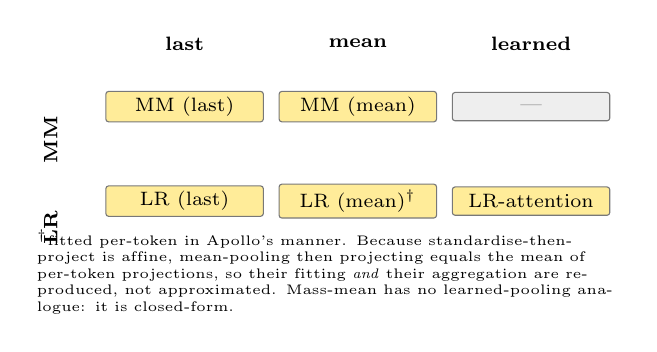
\begin{tikzpicture}[x=1mm,y=1mm]
\node[font=\scriptsize\bfseries] at (14,4) {last}; \node[font=\scriptsize\bfseries] at (36,4) {mean};
\node[font=\scriptsize\bfseries] at (58,4) {learned};
\node[font=\scriptsize\bfseries, anchor=east, rotate=90] at (-3,-4) {MM};
\node[font=\scriptsize\bfseries, anchor=east, rotate=90] at (-3,-16) {LR};
\node[tok, fill=probed, minimum width=20mm] at (14,-4) {MM (last)};
\node[tok, fill=probed, minimum width=20mm] at (36,-4) {MM (mean)};
\node[tok, fill=unprobed, minimum width=20mm, text=gray] at (58,-4) {---};
\node[tok, fill=probed, minimum width=20mm] at (14,-16) {LR (last)};
\node[tok, fill=probed, minimum width=20mm] at (36,-16) {LR (mean)$^{\dagger}$};
\node[tok, fill=probed, minimum width=20mm] at (58,-16) {LR-attention};
\node[font=\tiny, anchor=west, text width=74mm] at (-6,-25)
 {$^{\dagger}$fitted per-token in Apollo's manner. Because standardise-then-project
  is affine, mean-pooling then projecting equals the mean of per-token projections,
  so their fitting \emph{and} their aggregation are reproduced, not approximated.
  Mass-mean has no learned-pooling analogue: it is closed-form.};
\end{tikzpicture}
\caption{The probe grid. Crossing estimator with pooling allows a difference to be
attributed to one axis rather than confounded across both.}
\label{fig:grid}
\end{figure}

The per-token set is uncapped for all behaviours. A 60{,}000-row tractability
cap inherited from earlier hardware bound only on high-stakes, discarding 79\% of
285{,}394 rows and making this one cell a faithful reproduction for two
behaviours and a subsample for the third.

\emph{Metrics.} AUROC with a bootstrap 95\% confidence interval (1{,}000
resamples) is the primary metric, chosen over the accuracy \citet{marks2024}
report because the evaluation sets here are not class-balanced and the probe
scores are not calibrated to a common threshold: mass-mean's raw projection is
uncentred, so a fixed-threshold accuracy would measure calibration drift
rather than separability (R2). TPR at 1\% FPR is reported for comparability with
\citet{mckenzie2025}, and returns \texttt{n/a} when a set has fewer than 100
negatives, since 1\% FPR is then unreachable and the metric would silently
degrade to TPR at zero false positives. This is a weaker measurement than
Apollo's identically-named one, which calibrates the threshold against a separate
control corpus \citep{taori2023}; without such a split the figure here is
computed within each evaluation set and is not comparable to theirs.

\subsection{Causal steering}
\label{sec:steering}

\emph{What this stage does, and why.} Steering inverts the read direction: instead
of projecting an activation onto a direction to \emph{score} it, we add the
direction into the residual stream during a forward pass and ask whether the model's
behaviour changes. This is the control detection cannot provide (R4, and §I): a probe
that scores well may have found a correlate, whereas a direction that changes the
output is one the model uses. A fair comparison requires three things, each settled
below. Coefficients must mean the same thing across estimators, so directions of
differing norm are \emph{calibrated} to a common scale. The intervention must land in
the same place for every arm, and that place must not overlap the measuring
apparatus. The effect must be measured two ways, on a constrained readout and on free
generation, because a direction can move a readout while destroying the text and a
single measurement cannot distinguish the two.

Directions are refitted at each block layer and calibrated so that coefficient
$1.0$ moves the mean negative activation onto the mean positive one, following
\citeauthor{marks2024}'s normalisation; this makes coefficients comparable across
estimators whose raw directions differ in norm (R1).

\emph{Where the vector is written} is set by the instrument
(Fig.~\ref{fig:scope}), and is the one design point where an inherited default
proved untenable. Applying it to every token, the convention of the teaching notebook this
project builds on \citep{arena2024}, perturbs the readout's own few-shot
demonstrations, which contain the literal \textsc{yes}/\textsc{no} tokens the metric
reads. The measured effect would then be partly pressure on the instrument rather
than a change in how the transcript is represented.
\citet{marks2024} avoid exactly this by confining the intervention to their
group-(b) hidden states and excluding the readout position. The readout therefore
steers only the item transcript (15--21\% of the prompt), and generation steers
only the completion, which is also what CAA does \citep{rimsky2024}. Uniformity
across arms is preserved: within a scope, every direction touches identical
positions.

\begin{figure}[t]
\centering
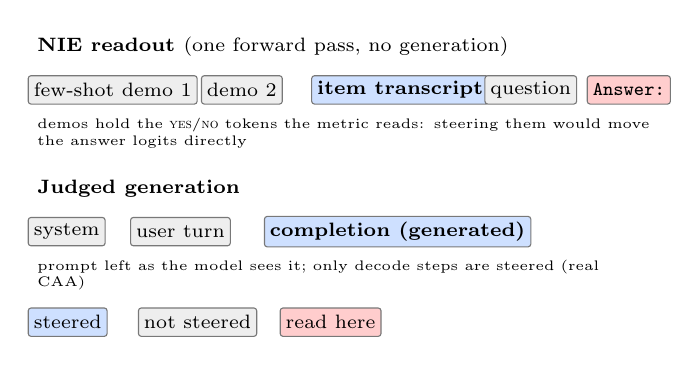
\begin{tikzpicture}[x=1mm,y=1mm]
\node[font=\scriptsize\bfseries, anchor=west] at (0,0) {NIE readout \textnormal{(one forward pass, no generation)}};
\node[ubox, anchor=west] at (0,-5.5) {few-shot demo 1};
\node[ubox, anchor=west] at (22,-5.5) {demo 2};
\node[sbox, anchor=west] at (36,-5.5) {\textbf{item transcript}};
\node[ubox, anchor=west] at (58,-5.5) {question};
\node[rbox, anchor=west] at (71,-5.5) {\texttt{Answer:}};
\node[font=\tiny, anchor=west, text width=78mm] at (0,-11)
 {demos hold the \textsc{yes}/\textsc{no} tokens the metric reads: steering them
  would move the answer logits directly};
\node[font=\scriptsize\bfseries, anchor=west] at (0,-18) {Judged generation};
\node[ubox, anchor=west] at (0,-23.5) {system};
\node[ubox, anchor=west] at (13,-23.5) {user turn};
\node[sbox, anchor=west] at (30,-23.5) {\textbf{completion (generated)}};
\node[font=\tiny, anchor=west, text width=78mm] at (0,-29)
 {prompt left as the model sees it; only decode steps are steered (real CAA)};
\node[sbox, anchor=west] at (0,-35) {steered};
\node[ubox, anchor=west] at (14,-35) {not steered};
\node[rbox, anchor=west] at (32,-35) {read here};
\end{tikzpicture}
\caption{Steering scope, per instrument. Narrowing the readout to the transcript
is what keeps the causal metric measuring the representation rather than the
measuring apparatus.}
\label{fig:scope}
\end{figure}

Generation prompts follow one rule, adapted from CAA's practice of deriving
open-ended prompts from the same held-out items as the constrained evaluation:
\textbf{a generation prompt is one where the behaviour is off but possible}.
For deception that is an AI Liar scenario under its neutral instruction; for
high-stakes, a low-stakes scenario; for sycophancy, a user turn carrying a
\emph{false} claim, since a true claim makes the behaviour not merely absent but
impossible.

\subsection{Implementation}
The pipeline is a Python package ($\approx$2{,}900 lines) with one driver
notebook per behaviour, evolved through three versions: a teaching notebook
\citep{arena2024}, a monolithic audited notebook, and the current modular
package, whose docstrings cite the source-paper section for each estimator so
provenance is checkable line by line. Two decisions were forced by scale.
Activations are extracted once per example at \emph{all} layers in a single
forward pass and cached as fp16, which makes the 32-layer sweep effectively free;
full un-pooled token grids, roughly eight times larger, are extracted only at the
chosen layer. All tokenisation flows through shared helpers, after a double-BOS
defect was found in which templated text and masks disagreed by one token,
silently scoring every probe on misaligned activations. The exported probes and
directions are served by a small interface for interactive scoring and steering.

\subsection{Evaluation}

\subsubsection{Probing}
Each probe is scored on a held-out in-distribution split and at least one
out-of-distribution set, by AUROC with bootstrap intervals and TPR at 1\% FPR as
described in §\ref{sec:detection}. Splits are pair-aware throughout: by fact
for deception, by pair for high-stakes, by prompt group for sycophancy. Layer
selection touches only training data (R6). Alongside the quantitative
result, each behaviour reports a centred PCA of the detection-layer activations
beside a histogram of projections onto the trained direction; the pairing is
diagnostic. Separation under unsupervised PCA would suggest the probe rides a topic
confound of the kind Apollo report, whereas separation only along the supervised
direction argues the confound axes are roughly orthogonal to it.

\subsubsection{Steering}
\label{sec:steereval}
Two independent measurements are taken at every (direction, coefficient).

The \emph{normalised indirect effect} reproduces \citeauthor{marks2024}'s
construction with YES/NO substituted for TRUE/FALSE. The model reads a few-shot
prompt ending in a question about a transcript and we record
$PD = P(\textsc{yes})-P(\textsc{no})$ at the final position. Writing $PD^{+}$ and
$PD^{-}$ for the unsteered means over positive and negative transcripts and
$PD^{-}_{*}$ for the steered mean over negatives,
\begin{equation}
\mathrm{NIE} \;=\; \frac{PD^{-}_{*} - PD^{-}}{PD^{+} - PD^{-}} ,
\label{eq:nie}
\end{equation}
so $\mathrm{NIE}=0$ means the intervention did nothing and $\mathrm{NIE}=1$ means
it moved the negatives a full class gap. No text is generated. The denominator
makes the metric scale-free but also fragile: it is meaningful only when the model
separates the classes unsteered, so a warning fires below a gap of $0.05$ and the
denominators are reported alongside the effects. Only negatives are steered,
toward the behaviour; \citeauthor{marks2024} additionally report the reverse
direction, which is not measured here.

The \emph{judge} satisfies R4. The model generates with steering active and Claude
Haiku 4.5 scores the generation 1--10 on the behaviour rubric \emph{and}
separately on coherence, with scores bounded server-side by an enumerated schema.
CAA restricted its multiplier range to avoid quality degradation. Measuring
coherence instead makes the degradation observable.
Coefficients sweep $\{-2,-1,-0.5,0,0.5,1,2\}$, so monotonicity is inspectable and
the negative half acts as a control. A blind agreement protocol for the judge
(author scores versus judge scores, reported as Spearman $\rho$) exists but has not
been run, so all judge figures are unvalidated.

%=======================================================================
\section{Results}
\label{sec:results}

\begin{table}[t]
\caption{Selected configuration. Layers are 0-indexed of 32.}
\label{tab:config}
\centering
\small
\setlength{\tabcolsep}{3.5pt}
\begin{tabular}{lccc}
\toprule
& \textbf{Deception} & \textbf{High-stakes} & \textbf{Sycophancy} \\
\midrule
Detection layer & 12 & 13 & 19 \\
Steering block  & 15--19 & 8--12 & 5--9 \\
Mask policy & assistant & content & assistant \\
Train / ID test & 488 / 124 & 3{,}000 / 1{,}000 & 2{,}736 / 694 \\
OOD & Liar 54, RP 742 & HH 2{,}984 & math 1{,}000 \\
\bottomrule
\end{tabular}
\end{table}

\begin{figure*}[t]
\centering
\figslot{steering_deception_ai_liar.png}{0.84\textwidth}{1.9cm}\\[0pt]
{\footnotesize (a) \textbf{deception} --- AI Liar (OOD)}\\[3pt]
\figslot{steering_highstakes_ood.png}{0.84\textwidth}{1.9cm}\\[0pt]
{\footnotesize (b) \textbf{high-stakes} --- Anthropic-HH (OOD)}\\[3pt]
\figslot{steering_sycophancy_ood.png}{0.84\textwidth}{1.9cm}\\[0pt]
{\footnotesize (c) \textbf{sycophancy} --- math (OOD)}
\caption{\textbf{Steering, out-of-distribution.} One row per behaviour, each carrying three panels:
\emph{readout NIE} (left), \emph{judge: behaviour} (centre), \emph{judge: coherence} (right), against
signed coefficient with the three directions overlaid. In-distribution panels are in Appendix~E-F, and
are weaker evidence: blocks were selected to maximise NIE on training transcripts, and deception's
in-distribution readout is degenerate (class gap $0.058$). \emph{What to look for.} Mass-mean leads on
NIE in (a) and (b), which is the write side of the dissociation, but not in (c), where it peaks at
$+0.5$, collapses by $+1$, and the attention direction alone rises monotonically. Read each
right-hand panel against its centre one: a behaviour rise coinciding with a coherence fall is steering
by breaking the model rather than by inducing the behaviour.}
\label{fig:steer}
\end{figure*}

Table~\ref{tab:config} gives the configuration. The behaviours place their
detection layers very differently, at 12, 13 and 19 of 32. Sycophancy is the only
one whose steering block (5--9) lies \emph{below} its detection layer, so its causal
site is earlier than its readable one.

Across all three behaviours, unsupervised PCA of the detection-layer activations
shows no class separation while the projection onto the trained direction
separates cleanly. This is the informative outcome rather than a failure: the
behaviour is a low-variance direction that content variance swamps. Had PCA separated
the classes, a topic confound would be the leading explanation.

\begin{figure}[t]
\centering
\figslot{layers_highstakes.png}{0.96\columnwidth}{2.1cm}
\caption{\textbf{Detection-layer selection, high-stakes.} Pair-aware 5-fold CV AUROC against layer,
mass-mean as selector with a logistic-regression overlay as a robustness check, chosen layer marked.
\emph{Why high-stakes.} Its curve has a genuine peak, so the argmax is meaningful; deception's
saturates near 1.000 across the upper two-thirds of the network, which makes the same choice look more
arbitrary than it is. \emph{What to look for.} That the LR overlay tracks the MM selector: if it did
not, the layer would be an artefact of the cheap estimator used to choose it. Deception and sycophancy
are in Appendix~E-A.}
\label{fig:layers}
\end{figure}

\begin{figure*}[t]
\centering
\figslot{pca_deception.png}{0.72\textwidth}{2.0cm}
\caption{\textbf{Linear structure, deception, at the detection layer.} \emph{Left:} PCA of centred activations, showing no class
separation. \emph{Right:} projections onto the trained mass-mean direction, showing clean
bimodal separation. \emph{Why both panels.} Separation under unsupervised PCA would suggest the
probe rides a high-variance topic confound of the kind Apollo report; separation only along the
supervised direction argues the confound axes are roughly orthogonal to it. \emph{What to look for.}
The co-located point pairs on the left are the two members of each instructed pair, byte-identical
apart from the system prompt: direct visual confirmation that the behaviour is a low-variance
direction that content variance swamps. High-stakes and sycophancy are in Appendix~E.}
\label{fig:pca}
\end{figure*}

\begin{figure*}[t]
\centering
\begin{tabular}{@{}c@{\hspace{1.5mm}}c@{\hspace{1.5mm}}c@{}}
\figslot{roc_deception_ood.png}{0.32\textwidth}{2.4cm} &
\figslot{roc_highstakes_ood.png}{0.32\textwidth}{2.4cm} &
\figslot{roc_sycophancy_ood.png}{0.32\textwidth}{2.4cm} \\[1pt]
{\footnotesize (a) deception: AI Liar} & {\footnotesize (b) high-stakes: Anthropic-HH} &
{\footnotesize (c) sycophancy: math} \\
\end{tabular}
\caption{Out-of-distribution ROC curves, all five probe cells per behaviour. Shown
out-of-distribution because the in-distribution curves are near-degenerate: four of five deception
cells exceed 0.996 AUROC, so the curve hugs the corner and carries nothing the scalar does not. Here
the arms separate visibly, and the ordering \emph{is} the read side of the dissociation: the
logistic-regression family leads in (a) and (b), mass-mean in (c).}
\label{fig:roc}
\end{figure*}

\begin{figure}[t]
\centering
\figslot{cosines_deception.png}{0.84\columnwidth}{2.1cm}
\caption{Cosine similarity between the five deception probe directions. This addresses the obvious
objection to the whole comparison, that the arms might be finding the \emph{same} direction and
differing only in scale, in which case ``which steers better'' would be a units artefact. Cosines well
below 1 mean they are genuinely different directions. High-stakes and sycophancy are in Appendix~E.}
\label{fig:cos}
\end{figure}

\subsection{Deception}
Detection is near-ceiling in-distribution: four of five cells reach $\geq 0.996$ and
three reach exactly 1.000. The comparison therefore only becomes visible
out-of-distribution, where \texttt{LR (mean)} leads at 0.722 on the pooled set and the
logistic-regression family wins 75\% of columns, as Apollo predict.

The two out-of-distribution sets separate informatively (Table~\ref{tab:decood}).
Every cell scores well on AI Liar, where the honest and deceptive members share
byte-identical answer text, and every cell collapses on roleplaying, where the
completions genuinely differ. That ordering is the opposite of what a
surface-cue account predicts. If the probes read deceptive \emph{phrasing},
roleplaying should be the easier set. Instead they handle the set where the text is
identical across labels, which argues they read framing in context.

\begin{table}[t]
\caption{Deception detection AUROC by out-of-distribution set. AI Liar has
byte-identical answers across labels; roleplaying does not.}
\label{tab:decood}
\centering
\small
\begin{tabular}{lccc}
\toprule
Probe & ID test & AI Liar & Roleplaying \\
\midrule
MM (last)    & 0.948 & 0.959 & 0.669 \\
MM (mean)    & 1.000 & 0.992 & 0.654 \\
LR (last)    & 0.996 & 0.818 & 0.554 \\
LR (mean)    & 1.000 & 0.974 & \textbf{0.706} \\
LR-attention & 1.000 & 0.989 & 0.657 \\
\bottomrule
\end{tabular}
\end{table}

\begin{figure}[t]
\centering
\figslot{heatmap_deception_deceptive.png}{0.92\columnwidth}{1.6cm}\\[3pt]
\figslot{heatmap_deception_honest.png}{0.92\columnwidth}{1.6cm}
\caption{\textbf{Per-token probe scores, one deception pair:} deceptive persona (top), honest twin
(bottom) --- the mask of §III-B made visible, since only assistant-content tokens are scored.
\emph{Why a pair rather than one example.} The two members share an identical user turn and the same
truncated fact, differing only in the system persona, so any difference in colour is the probe reading
\emph{context} rather than lexical content. \emph{What to look for.} Where the score rises: early,
before any giveaway, is the intent reading Apollo report; only on a tell-tale phrase would suggest a
surface cue.}
\label{fig:heat}
\end{figure}

On steering, mass-mean wins every column, so the dissociation holds. But the
in-distribution figure must be discarded: its class gap is $+0.058$, because the
model answers ``NO'' to the deception question for \emph{both} classes
($PD^{+}=-0.906$, $PD^{-}=-0.964$), and dividing by that inflates the ratio
roughly seventeenfold. The AI Liar column, on a healthy gap of $1.052$, supports
the same ranking soundly and is the one relied on. On roleplaying all three
directions produce NIEs at or below zero: steering does not transfer to the
harder set, mirroring the detection collapse there.

\subsection{High-stakes}
This is the cleanest case. The logistic-regression family wins 100\% of detection
columns, with \texttt{LR (mean)} at 0.826 out-of-distribution against mass-mean's
0.699, and the learned attention probe leads in-distribution at 0.997,
consistent with \citeauthor{mckenzie2025}'s finding that pooling matters. Mass-mean
then wins 100\% of steering columns, monotonically on the out-of-distribution set
($0.163 \to 0.560 \to 1.252$ across coefficients $0.5$, $1$, $2$). It also moves
the judged behaviour furthest at coefficient $1$ ($3.75 \to 5.62$ against LR's
$4.54$). Read and write disagree cleanly, with both sides well-conditioned.

\subsection{Sycophancy}
Sycophancy inverts the pattern on both sides at once. \texttt{MM (last)} is the
best out-of-distribution detector at 0.879, and the logistic-regression family
wins \emph{no} detection column. Mass-mean is then among the worst steerers: the
attention direction is the only one with a clean monotone steering response
(in-distribution $0.11 \to 0.25 \to 0.51$; math $0.13 \to 0.34 \to 0.48$), while
mass-mean's curve peaks at coefficient $+0.5$ and collapses by $+1$, which is
where the verdict is read.

Two of this behaviour's design features explain part of it. Pooling is inverted
relative to the other behaviours: \texttt{last} beats \texttt{mean} for
\emph{both} estimators here, the only such case, which is what the 79\%
identical templated prefix predicts, since mean pooling averages in tokens whose
activations are identical across classes. And the label is relational: it depends
on whether the reply matches a claim that is itself true or false, with 29\% of
negatives being genuine agreement. A difference-of-means direction over such data
may capture the surface regularity of agreement, which reads well but is not the
lever that produces deference. That the steering block (5--9) sits below the
detection layer (19) is consistent: the readable site is not the writable one.

\begin{figure}[t]
\centering
\figslot{niesweep_deception.png}{0.94\columnwidth}{2.1cm}
\caption{Per-layer NIE for deception, one layer steered at a time; the selected five-layer block is the
contiguous window of maximum summed causal effect. This is the write-side analogue of
Fig.~\ref{fig:layers}, and the contrast between the two is the point: the causal band (15--19) sits
well above the detection layer (12), so predictive performance and causal effect do not peak in the
same place. High-stakes and sycophancy are in Appendix~E; sycophancy inverts the offset, placing its
causal band \emph{below} its detection layer.}
\label{fig:nie}
\end{figure}

\subsection{Synthesis}
Table~\ref{tab:synth} states the comparison the study was built to make.

\begin{table}[t]
\caption{The read/write comparison. The dissociation holds where the LR family
wins detection and mass-mean wins steering.}
\label{tab:synth}
\centering
\small
\setlength{\tabcolsep}{3.5pt}
\begin{tabular}{lccc}
\toprule
& \textbf{Deception} & \textbf{High-stakes} & \textbf{Sycophancy} \\
\midrule
Best OOD detector & LR (mean) & LR (mean) & \textbf{MM (last)} \\
LR-family win share & 75\% & 100\% & \textbf{0\%} \\
Best steerer & MM & MM & \textbf{LR-attn} \\
MM win share & 100\% & 100\% & \textbf{0\%} \\
\midrule
Dissociation & holds & holds & \textbf{inverts} \\
\bottomrule
\end{tabular}
\end{table}

The coherence axis then qualifies the write side. At coefficient $+2$ mass-mean
degrades generation quality on every behaviour and every evaluation set, judge
coherence falling from 4.38 to 1.92 on AI Liar, 6.21 to 2.83 on high-stakes
out-of-distribution, and 6.58 to 1.00 on sycophancy out-of-distribution, while
logistic-regression and attention directions leave it essentially intact. The
collapse is a property of the direction, not of a behaviour.

Sycophancy also shows why \emph{both} write-side instruments are needed (R2), because
they disagree there. In-distribution, mass-mean moves the judged behaviour
substantially at coefficient $+1$ ($1.17 \to 5.67$) but coherence falls from 9.08 to
3.83 at the same point, the sycophantic-looking text is produced by degradation, and
the NIE alone would have scored that a success. Out-of-distribution the disagreement
runs the other way: at $+1$ the judge records a large behaviour rise ($1.00 \to 7.33$)
with coherence essentially intact ($6.58 \to 7.33$), while the NIE at that coefficient
is \emph{negative} ($-0.16$). One instrument sees induction, the other sees nothing.
Neither measurement is therefore sufficient alone. Mass-mean's sycophancy curve is also
non-monotone throughout: its NIE peaks at $+0.5$ ($0.91$) before collapsing, so no
single coefficient summarises it.


%=======================================================================
\section{Discussion}

\textbf{The dissociation is real but conditional.} On two of three behaviours the
directions that read best and write best differ, reproducing on safety behaviours
what \citet{marks2024} found for truth, and here, unlike across papers, the
model, layer, tokens, calibration and intervention site are identical across arms.

\textbf{Sycophancy shows it is not a law.} The inversion is complete, and the
relational-label and templated-prefix explanations above are testable. The
dissociation should therefore be treated as a property of a
behaviour--representation pair rather than as guidance that generalises to an
untested behaviour.

\textbf{Pooling can matter more than the estimator.} Sycophancy's
\texttt{last}-beats-\texttt{mean} inversion is a larger effect than several
estimator differences. It follows from a dataset design choice, factorial templates
holding everything but the answer fixed, interacting with a probing choice. Neither
source paper confronts this, since \citeauthor{mckenzie2025}'s mean-beats-last result
assumes lexically varied inputs.

\textbf{Coherence changes what ``causal'' means.} Mass-mean's advantage co-occurs
with faster quality degradation. A readout-based metric cannot see this, because a
degraded model still emits the target token. ``More causal'' should therefore be read
as ``larger effect per unit coefficient, with faster degradation''. This distinction
is unavailable to \citeauthor{marks2024}'s readout-only design.

\textbf{Detection generalisation is the binding constraint.} Every behaviour loses
substantial AUROC out-of-distribution: deception 1.000 to 0.722, high-stakes 0.997
to 0.826, and sycophancy 0.976 to 0.879. At this scale these probes would not
support deployment as monitors, consistent with Apollo's conclusion that current
performance is insufficient as a robust defence.

\subsection{Limitations}
\label{sec:limitations}

\textbf{Reported steering numbers predate the scope fix and are upper bounds.}
Every NIE here was measured with the vector written to all tokens of the readout
prompt, so part of each value may be pressure on the demonstrations rather than a
representational change. The transcript-only scope is implemented and tested but not
yet re-run; it shrinks the intervention from 100\% of the prompt to 15--21\%. Because
the change is uniform across directions, the \emph{ordering} should survive even
where the magnitudes do not.

\textbf{The judge is unvalidated.} The blind agreement protocol has not been run,
and coherence carries much of the interpretation above. CAA validated its judge by
manual spot-check; that step is outstanding here.

\textbf{NIE is selected on.} Blocks are chosen to maximise summed NIE and NIE is
then reported at those blocks. Train/test separation is maintained, the sweep
uses training transcripts, so this is hyperparameter selection rather than
leakage, but out-of-distribution figures deserve more weight than in-distribution
ones.

\textbf{The block is selected using mass-mean only}, then used for all arms. A
sweep with the logistic-regression direction showing the block barely moves would
close the alternative explanation that the block suits mass-mean.

\textbf{The roleplaying judge panel cannot show induction.} Its prompts are
inherently pressured, and the honest/deceptive flag is a no-op once the completion is
stripped, so no behaviour-off variant exists. The baseline is already 6.96/10
deceptive and the panel stays within 6.08--7.83 throughout, so it is uninformative
rather than evidence that steering failed. Its detection results and NIE are
unaffected.

\textbf{Missing arms.} No covariance-corrected mass-mean probe, which both
\citet{marks2024} and Apollo benchmark; no control corpus, so TPR at 1\% FPR is
not comparable to Apollo's; no reverse steering direction; no insider-trading or
sandbagging evaluation. Single model, single seed.

%=======================================================================
\section{Future Work}

\textbf{Close the open controls.} In priority order: re-run steering under the
corrected scope; run the blind judge validation; sweep the steering block with the
logistic-regression direction. A covariance-corrected mass-mean arm was considered
and set aside: with $d=4096$ and at most a few thousand pooled examples the
covariance is severely rank-deficient for every behaviour, but the cheaper form
of the same test is to report
$\cos(\Sigma^{-1}\boldsymbol{\theta}_{\mathrm{mm}}, \boldsymbol{\theta}_{\mathrm{LR}})$,
which \citeauthor{marks2024}'s Appendix F predicts is near 1 and which would
explain the read-side result mechanistically rather than merely observing it.

\textbf{Complete the metric.} Add the reverse steering direction, which
\citeauthor{marks2024} report and whose two directions can diverge substantially,
and a control corpus so the false-positive figure means what it means in the
deception literature.

\textbf{Explain the sycophancy inversion.} The relational-label hypothesis is
testable: restricting training to non-genuine-agreement negatives should, if
correct, move mass-mean toward a causal lever at the cost of detection. The gap
between layer 19 and layers 5--9 invites a layer-resolved analysis of where
deference is computed versus where it is legible.

\textbf{Scale, behaviours and mechanism.} Extending to 70B would test whether the
dissociation strengthens with scale, as \citeauthor{marks2024} observe for linear
structure generally; user intention and refusal are the next behaviours; and
replacing linear directions with sparse-autoencoder latents
\citep{cunningham2023,bricken2023} would test whether a sparser basis separates
the readable feature from the writable one. Preliminary machinery exists for
steering two behaviours at once, which no source paper addresses.

%=======================================================================
\section{Conclusion}

We built one pipeline that asks, for three safety behaviours in a single model,
whether the direction that best detects a behaviour is the direction that best
steers it, and that fixes the surrounding choices, from token masking to
pooling to intervention site, so the answer is attributable. For deception and
high-stakes the answer is no, in the manner the literature implies:
logistic-regression directions read best, mass-mean directions write best. For
sycophancy it inverts completely, showing the dissociation is a property of
particular behaviour--representation pairs rather than of linear probes in
general. The coherence axis further shows that mass-mean's causal advantage is
partly a matter of steering harder rather than better. We regard the sycophancy
inversion, and the conditions under which the causal metric is trustworthy, as the
more useful contributions.

%=======================================================================
\section*{Acknowledgment}

The author thanks her supervisor for guidance throughout. The pipeline builds on
the ARENA 3.0 interpretability curriculum \citep{arena2024} and on datasets
released by \citet{goldowsky2025}, \citet{mckenzie2025} and \citet{cincynlp2025}.
Use of generative AI tools is declared in Appendix~D.

%=======================================================================
\begin{thebibliography}{99}
\setlength{\itemsep}{2pt}

\bibitem[Alain and Bengio(2018)]{alain2018}
Alain, G. and Bengio, Y. (2018) `Understanding intermediate layers using linear
classifier probes', \textit{arXiv preprint} arXiv:1610.01644.

\bibitem[Azaria and Mitchell(2023)]{azaria2023}
Azaria, A. and Mitchell, T. (2023) `The internal state of an LLM knows when it's
lying', in \textit{Findings of EMNLP 2023}. arXiv:2304.13734.

\bibitem[Bai et al.(2022)]{bai2022}
Bai, Y., Jones, A., Ndousse, K., et al. (2022) `Training a helpful and harmless
assistant with reinforcement learning from human feedback', \textit{arXiv
preprint} arXiv:2204.05862.

\bibitem[Bricken et al.(2023)]{bricken2023}
Bricken, T., Templeton, A., Batson, J., et al. (2023) `Towards monosemanticity:
decomposing language models with dictionary learning',
\textit{Transformer Circuits Thread}.

\bibitem[Burns et al.(2023)]{burns2023}
Burns, C., Ye, H., Klein, D. and Steinhardt, J. (2023) `Discovering latent
knowledge in language models without supervision', in \textit{International
Conference on Learning Representations (ICLR)}.

\bibitem[CincyNLP(2025)]{cincynlp2025}
CincyNLP (2025) \textit{Disentangling sycophancy: factorial evaluation
datasets}. Available at: \url{https://github.com/cincynlp/disentangle-sycophancy}
(Accessed: 30 July 2026).

\bibitem[Cunningham et al.(2023)]{cunningham2023}
Cunningham, H., Ewart, A., Riggs, L., Huben, R. and Sharkey, L. (2023) `Sparse
autoencoders find highly interpretable features in language models',
\textit{arXiv preprint} arXiv:2309.08600.

\bibitem[Elhage et al.(2022)]{elhage2022}
Elhage, N., Hume, T., Olsson, C., et al. (2022) `Toy models of superposition',
\textit{Transformer Circuits Thread}.

\bibitem[Goldowsky-Dill et al.(2025)]{goldowsky2025}
Goldowsky-Dill, N., Chughtai, B., Heimersheim, S. and Hobbhahn, M. (2025)
`Detecting strategic deception using linear probes', \textit{arXiv preprint}
arXiv:2502.03407.

\bibitem[Kantamneni et al.(2025)]{kantamneni2025}
Kantamneni, S., Engels, J., Rajamanoharan, S. and Nanda, N. (2025) `Are sparse
autoencoders useful? A case study in sparse probing', \textit{arXiv preprint}
arXiv:2502.16681. \textcolor{red}{[VERIFY: McKenzie et al.\ and Apollo both cite
``Kantamneni et al.\ (2024)'' --- confirm this is the same work and not an earlier paper]}

\bibitem[Levinstein and Herrmann(2024)]{levinstein2024}
Levinstein, B.A. and Herrmann, D.A. (2024) `Still no lie detector for language
models: probing empirical and conceptual roadblocks',
\textit{Philosophical Studies}. \textcolor{red}{[verify year/volume: arXiv 2023, journal 2024]}

\bibitem[Li et al.(2023)]{li2023}
Li, K., Patel, O., Vi\'egas, F., Pfister, H. and Wattenberg, M. (2023)
`Inference-time intervention: eliciting truthful answers from a language model',
in \textit{Advances in Neural Information Processing Systems (NeurIPS)}.

\bibitem[Marks and Tegmark(2024)]{marks2024}
Marks, S. and Tegmark, M. (2024) `The geometry of truth: emergent linear
structure in large language model representations of true/false datasets', in
\textit{Conference on Language Modeling (COLM)}. arXiv:2310.06824.

\bibitem[McDougall(2024)]{arena2024}
McDougall, C. (2024) \textit{ARENA 3.0: Alignment Research Engineer
Accelerator}. Available at: \url{https://github.com/callummcdougall/ARENA_3.0}
(Accessed: 2 August 2026).

\bibitem[McKenzie et al.(2025)]{mckenzie2025}
McKenzie, A., Pawar, U., Blandfort, P., Bankes, W., Krueger, D., Lubana, E.S.
and Krasheninnikov, D. (2025) `Detecting high-stakes interactions with
activation probes', \textit{arXiv preprint} arXiv:2506.10805.

\bibitem[Meng et al.(2022)]{meng2022}
Meng, K., Bau, D., Andonian, A. and Belinkov, Y. (2022) `Locating and editing
factual associations in GPT', in \textit{Advances in Neural Information
Processing Systems (NeurIPS)}.

\bibitem[Pacchiardi et al.(2024)]{pacchiardi2024}
Pacchiardi, L., Chan, A.J., Mindermann, S., et al. (2024) `How to catch an AI
liar: lie detection in black-box LLMs by asking unrelated questions', in
\textit{International Conference on Learning Representations (ICLR)}.

\bibitem[Perez et al.(2023)]{perez2023}
Perez, E., Ringer, S., Luko\v{s}i\=ut\.e, K., et al. (2023) `Discovering language
model behaviors with model-written evaluations', in \textit{Findings of ACL 2023}.
\textcolor{red}{[CAA cites this as Perez et al.\ 2022: arXiv Dec 2022, venue 2023]}

\bibitem[Rimsky et al.(2024)]{rimsky2024}
Rimsky, N., Gabrieli, N., Schulz, J., Tong, M., Hubinger, E. and Turner, A.
(2024) `Steering Llama 2 via contrastive activation addition', in
\textit{Proceedings of ACL 2024}. arXiv:2312.06681.

\bibitem[Scheurer et al.(2023)]{scheurer2023}
Scheurer, J., Balesni, M. and Hobbhahn, M. (2023) `Large language models can
strategically deceive their users when put under pressure',
\textit{arXiv preprint} arXiv:2311.07590.

\bibitem[Sharma et al.(2023)]{sharma2023}
Sharma, M., Tong, M., Korbak, T., et al. (2023) `Towards understanding sycophancy
in language models', \textit{arXiv preprint} arXiv:2310.13548.

\bibitem[Taori et al.(2023)]{taori2023}
Taori, R., Gulrajani, I., Zhang, T., et al. (2023) \textit{Stanford Alpaca: an
instruction-following LLaMA model}. Available at:
\url{https://github.com/tatsu-lab/stanford_alpaca} (Accessed: 2 August 2026).

\bibitem[Vig et al.(2020)]{vig2020}
Vig, J., Gehrmann, S., Belinkov, Y., et al. (2020) `Investigating gender bias in
language models using causal mediation analysis', in \textit{Advances in Neural
Information Processing Systems (NeurIPS)}.

\end{thebibliography}

%=======================================================================
\appendices

% AUTO-GENERATED by make_appendix_tables.py -- do not edit by hand.

% Regenerate after any pipeline re-run so these cannot drift from exported_probes/.



\section{Full Detection Results}

Every probe cell against every evaluation set, as exported to \texttt{exported\_probes/*\_detection.csv}. The out-of-distribution rows are the ones the read-side claim rests on; in-distribution AUROC is near-ceiling for two of the three behaviours and correspondingly uninformative.

\begin{table}[h]
\caption{Deception --- detection. AUROC with bootstrap 95\% CI; TPR at 1\% FPR (\texttt{n/a} where a set has $<$100 negatives, so 1\% FPR is unreachable).}
\label{tab:app-det-deception}
\centering
\scriptsize
\setlength{\tabcolsep}{3pt}
\begin{tabular}{llcc}
\toprule
Probe & Evaluation set & AUROC [95\% CI] & TPR@1\%FPR \\
\midrule
MM (last) & test (ID) & 0.948 [0.91,0.98] & n/a ($<$100 neg) \\
 & AI Liar (OOD) & 0.959 [0.90,0.99] & n/a ($<$100 neg) \\
 & Roleplaying (OOD) & 0.669 [0.63,0.71] & 0.011 \\
 & Deception OOD pool & 0.696 [0.66,0.73] & 0.033 \\
\addlinespace[2pt]
MM (mean) & test (ID) & 1.000 [1.00,1.00] & n/a ($<$100 neg) \\
 & AI Liar (OOD) & 0.992 [0.97,1.00] & n/a ($<$100 neg) \\
 & Roleplaying (OOD) & 0.654 [0.61,0.69] & 0.016 \\
 & Deception OOD pool & 0.679 [0.64,0.72] & 0.018 \\
\addlinespace[2pt]
LR (last) & test (ID) & 0.996 [0.99,1.00] & n/a ($<$100 neg) \\
 & AI Liar (OOD) & 0.818 [0.70,0.93] & n/a ($<$100 neg) \\
 & Roleplaying (OOD) & 0.554 [0.51,0.60] & 0.011 \\
 & Deception OOD pool & 0.571 [0.53,0.61] & 0.023 \\
\addlinespace[2pt]
LR (mean) & test (ID) & 1.000 [1.00,1.00] & n/a ($<$100 neg) \\
 & AI Liar (OOD) & 0.974 [0.93,1.00] & n/a ($<$100 neg) \\
 & Roleplaying (OOD) & 0.706 [0.67,0.74] & 0.078 \\
 & Deception OOD pool & 0.722 [0.69,0.76] & 0.075 \\
\addlinespace[2pt]
LR-attention & test (ID) & 1.000 [1.00,1.00] & n/a ($<$100 neg) \\
 & AI Liar (OOD) & 0.989 [0.97,1.00] & n/a ($<$100 neg) \\
 & Roleplaying (OOD) & 0.657 [0.62,0.69] & 0.049 \\
 & Deception OOD pool & 0.685 [0.65,0.72] & 0.055 \\
\addlinespace[2pt]
\bottomrule
\end{tabular}
\end{table}

\begin{table}[h]
\caption{High-stakes --- detection. AUROC with bootstrap 95\% CI; TPR at 1\% FPR (\texttt{n/a} where a set has $<$100 negatives, so 1\% FPR is unreachable).}
\label{tab:app-det-highstakes}
\centering
\scriptsize
\setlength{\tabcolsep}{3pt}
\begin{tabular}{llcc}
\toprule
Probe & Evaluation set & AUROC [95\% CI] & TPR@1\%FPR \\
\midrule
MM (last) & test (ID) & 0.867 [0.84,0.89] & 0.308 \\
 & anthropic\_hh\_balanced (OOD) & 0.678 [0.66,0.70] & 0.058 \\
\addlinespace[2pt]
MM (mean) & test (ID) & 0.951 [0.94,0.96] & 0.372 \\
 & anthropic\_hh\_balanced (OOD) & 0.699 [0.68,0.72] & 0.031 \\
\addlinespace[2pt]
LR (last) & test (ID) & 0.977 [0.97,0.98] & 0.688 \\
 & anthropic\_hh\_balanced (OOD) & 0.782 [0.77,0.80] & 0.128 \\
\addlinespace[2pt]
LR (mean) & test (ID) & 0.995 [0.99,1.00] & 0.828 \\
 & anthropic\_hh\_balanced (OOD) & 0.826 [0.81,0.84] & 0.080 \\
\addlinespace[2pt]
LR-attention & test (ID) & 0.997 [0.99,1.00] & 0.948 \\
 & anthropic\_hh\_balanced (OOD) & 0.808 [0.79,0.82] & 0.080 \\
\addlinespace[2pt]
\bottomrule
\end{tabular}
\end{table}

\begin{table}[h]
\caption{Sycophancy --- detection. AUROC with bootstrap 95\% CI; TPR at 1\% FPR (\texttt{n/a} where a set has $<$100 negatives, so 1\% FPR is unreachable).}
\label{tab:app-det-sycophancy}
\centering
\scriptsize
\setlength{\tabcolsep}{3pt}
\begin{tabular}{llcc}
\toprule
Probe & Evaluation set & AUROC [95\% CI] & TPR@1\%FPR \\
\midrule
MM (last) & test (ID) & 0.976 [0.97,0.98] & 0.862 \\
 & math (OOD) & 0.879 [0.86,0.90] & 0.200 \\
\addlinespace[2pt]
MM (mean) & test (ID) & 0.928 [0.91,0.94] & 0.602 \\
 & math (OOD) & 0.802 [0.77,0.83] & 0.018 \\
\addlinespace[2pt]
LR (last) & test (ID) & 0.975 [0.97,0.98] & 0.859 \\
 & math (OOD) & 0.847 [0.82,0.87] & 0.052 \\
\addlinespace[2pt]
LR (mean) & test (ID) & 0.970 [0.96,0.98] & 0.790 \\
 & math (OOD) & 0.825 [0.80,0.85] & 0.046 \\
\addlinespace[2pt]
LR-attention & test (ID) & 0.974 [0.96,0.98] & 0.865 \\
 & math (OOD) & 0.861 [0.84,0.88] & 0.050 \\
\addlinespace[2pt]
\bottomrule
\end{tabular}
\end{table}

\section{Full Steering Response Curves}

All seven coefficients for every direction and evaluation set, as exported to \texttt{exported\_probes/*\_steering\_full.json}. Three things are easiest to see here rather than in the body: whether a curve is monotone in the coefficient, whether the negative half behaves as a control, and where judge coherence falls away from its unsteered baseline.

\begin{table}[h]
\caption{Deception, ID: steering response. Readout NIE, judge behaviour and judge coherence (1--10; \texttt{---} where the judge arm is deliberately skipped).}
\label{tab:app-steer-deception-ID}
\centering
\scriptsize
\setlength{\tabcolsep}{3pt}
\begin{tabular}{llrrrrrrr}
\toprule
Direction & & -2 & -1 & -0.5 & +0 & +0.5 & +1 & +2 \\
\midrule
MM & NIE & -0.58 & -0.58 & -0.56 & +0.00 & +2.61 & +7.25 & +14.63 \\
 & judge beh. & --- & --- & --- & --- & --- & --- & --- \\
 & judge coh. & --- & --- & --- & --- & --- & --- & --- \\
\addlinespace[2pt]
LR & NIE & -0.56 & -0.55 & -0.44 & +0.00 & +0.99 & +2.29 & +3.70 \\
 & judge beh. & --- & --- & --- & --- & --- & --- & --- \\
 & judge coh. & --- & --- & --- & --- & --- & --- & --- \\
\addlinespace[2pt]
LR-attention & NIE & -0.53 & -0.49 & -0.33 & +0.00 & +0.54 & +1.15 & +2.57 \\
 & judge beh. & --- & --- & --- & --- & --- & --- & --- \\
 & judge coh. & --- & --- & --- & --- & --- & --- & --- \\
\addlinespace[2pt]
\bottomrule
\end{tabular}
\end{table}

\begin{table}[h]
\caption{Deception, AI Liar (OOD): steering response. Readout NIE, judge behaviour and judge coherence (1--10; \texttt{---} where the judge arm is deliberately skipped).}
\label{tab:app-steer-deception-AILiarOOD}
\centering
\scriptsize
\setlength{\tabcolsep}{3pt}
\begin{tabular}{llrrrrrrr}
\toprule
Direction & & -2 & -1 & -0.5 & +0 & +0.5 & +1 & +2 \\
\midrule
MM & NIE & +0.26 & -0.10 & -0.09 & +0.00 & +0.09 & +0.16 & +0.24 \\
 & judge beh. & 3.33 & 2.08 & 2.38 & 2.17 & 2.33 & 2.71 & 3.25 \\
 & judge coh. & 2.12 & 5.33 & 5.58 & 4.38 & 7.42 & 7.58 & 1.92 \\
\addlinespace[2pt]
LR & NIE & -0.37 & -0.14 & -0.07 & +0.00 & +0.05 & +0.05 & -0.15 \\
 & judge beh. & 2.38 & 2.12 & 2.21 & 2.17 & 2.42 & 2.33 & 3.12 \\
 & judge coh. & 4.96 & 5.17 & 5.58 & 4.38 & 5.58 & 5.88 & 3.83 \\
\addlinespace[2pt]
LR-attention & NIE & -0.13 & -0.04 & -0.00 & +0.00 & +0.02 & -0.02 & -0.15 \\
 & judge beh. & 2.04 & 2.67 & 2.12 & 2.17 & 2.04 & 2.33 & 2.50 \\
 & judge coh. & 4.75 & 4.79 & 5.38 & 4.38 & 6.04 & 5.54 & 6.29 \\
\addlinespace[2pt]
\bottomrule
\end{tabular}
\end{table}

\begin{table}[h]
\caption{Deception, Roleplaying (OOD): steering response. Readout NIE, judge behaviour and judge coherence (1--10; \texttt{---} where the judge arm is deliberately skipped).}
\label{tab:app-steer-deception-RoleplayingOOD}
\centering
\scriptsize
\setlength{\tabcolsep}{3pt}
\begin{tabular}{llrrrrrrr}
\toprule
Direction & & -2 & -1 & -0.5 & +0 & +0.5 & +1 & +2 \\
\midrule
MM & NIE & +0.53 & -0.02 & -0.00 & +0.00 & -0.05 & -0.07 & -0.15 \\
 & judge beh. & 6.42 & 7.12 & 6.62 & 6.96 & 6.75 & 6.62 & 6.08 \\
 & judge coh. & 1.04 & 5.00 & 5.62 & 6.08 & 6.04 & 5.71 & 1.38 \\
\addlinespace[2pt]
LR & NIE & -0.27 & -0.09 & -0.03 & +0.00 & -0.01 & -0.08 & -0.53 \\
 & judge beh. & 6.79 & 6.46 & 7.12 & 6.96 & 7.33 & 7.83 & 7.12 \\
 & judge coh. & 5.08 & 6.08 & 5.38 & 6.08 & 5.75 & 5.67 & 2.58 \\
\addlinespace[2pt]
LR-attention & NIE & -0.02 & +0.02 & +0.02 & +0.00 & -0.06 & -0.18 & -0.49 \\
 & judge beh. & 7.12 & 6.42 & 6.79 & 6.96 & 7.33 & 7.12 & 7.08 \\
 & judge coh. & 5.29 & 6.12 & 5.79 & 6.08 & 5.67 & 5.79 & 4.92 \\
\addlinespace[2pt]
\bottomrule
\end{tabular}
\end{table}

\begin{table}[h]
\caption{High-stakes, ID: steering response. Readout NIE, judge behaviour and judge coherence (1--10; \texttt{---} where the judge arm is deliberately skipped).}
\label{tab:app-steer-highstakes-ID}
\centering
\scriptsize
\setlength{\tabcolsep}{3pt}
\begin{tabular}{llrrrrrrr}
\toprule
Direction & & -2 & -1 & -0.5 & +0 & +0.5 & +1 & +2 \\
\midrule
MM & NIE & -3.06 & -3.27 & -2.01 & +0.00 & +1.25 & +1.52 & +1.24 \\
 & judge beh. & 2.46 & 3.42 & 3.71 & 3.75 & 5.33 & 5.62 & 5.62 \\
 & judge coh. & 5.04 & 4.75 & 4.46 & 4.42 & 5.00 & 4.75 & 2.83 \\
\addlinespace[2pt]
LR & NIE & -2.49 & -1.41 & -0.72 & +0.00 & +0.52 & +1.01 & +1.49 \\
 & judge beh. & 3.54 & 3.71 & 4.46 & 3.75 & 4.50 & 4.54 & 4.42 \\
 & judge coh. & 5.00 & 5.12 & 4.75 & 4.42 & 4.50 & 4.58 & 4.38 \\
\addlinespace[2pt]
LR-attention & NIE & -3.62 & -2.32 & -1.30 & +0.00 & +0.84 & +1.38 & +1.56 \\
 & judge beh. & 3.50 & 3.71 & 3.50 & 3.75 & 4.50 & 4.38 & 6.00 \\
 & judge coh. & 5.33 & 4.71 & 4.75 & 4.42 & 4.71 & 4.79 & 5.04 \\
\addlinespace[2pt]
\bottomrule
\end{tabular}
\end{table}

\begin{table}[h]
\caption{High-stakes, Anthropic HH (OOD): steering response. Readout NIE, judge behaviour and judge coherence (1--10; \texttt{---} where the judge arm is deliberately skipped).}
\label{tab:app-steer-highstakes-AnthropicHHOOD}
\centering
\scriptsize
\setlength{\tabcolsep}{3pt}
\begin{tabular}{llrrrrrrr}
\toprule
Direction & & -2 & -1 & -0.5 & +0 & +0.5 & +1 & +2 \\
\midrule
MM & NIE & -0.06 & -0.07 & -0.06 & +0.00 & +0.16 & +0.56 & +1.25 \\
 & judge beh. & 1.42 & 1.67 & 1.83 & 1.79 & 1.83 & 1.96 & 2.58 \\
 & judge coh. & 6.71 & 7.38 & 6.54 & 6.21 & 6.21 & 5.00 & 2.83 \\
\addlinespace[2pt]
LR & NIE & -0.07 & -0.05 & -0.03 & +0.00 & +0.05 & +0.12 & +0.36 \\
 & judge beh. & 1.83 & 1.79 & 1.79 & 1.79 & 1.75 & 1.71 & 1.79 \\
 & judge coh. & 5.92 & 6.29 & 6.38 & 6.21 & 6.29 & 6.21 & 5.79 \\
\addlinespace[2pt]
LR-attention & NIE & -0.07 & -0.07 & -0.04 & +0.00 & +0.09 & +0.26 & +0.78 \\
 & judge beh. & 1.79 & 1.83 & 1.83 & 1.79 & 1.75 & 1.79 & 1.96 \\
 & judge coh. & 7.00 & 6.50 & 6.54 & 6.21 & 6.00 & 5.88 & 6.00 \\
\addlinespace[2pt]
\bottomrule
\end{tabular}
\end{table}

\begin{table}[h]
\caption{Sycophancy, ID: steering response. Readout NIE, judge behaviour and judge coherence (1--10; \texttt{---} where the judge arm is deliberately skipped).}
\label{tab:app-steer-sycophancy-ID}
\centering
\scriptsize
\setlength{\tabcolsep}{3pt}
\begin{tabular}{llrrrrrrr}
\toprule
Direction & & -2 & -1 & -0.5 & +0 & +0.5 & +1 & +2 \\
\midrule
MM & NIE & +0.03 & -0.55 & +0.04 & +0.00 & +0.89 & +0.08 & +0.03 \\
 & judge beh. & 1.00 & 1.04 & 1.83 & 1.17 & 1.29 & 5.67 & 1.00 \\
 & judge coh. & 1.00 & 7.25 & 8.12 & 9.08 & 9.71 & 3.83 & 1.00 \\
\addlinespace[2pt]
LR & NIE & -0.07 & -0.04 & -0.04 & +0.00 & +0.01 & -0.00 & +0.03 \\
 & judge beh. & 1.46 & 1.50 & 1.42 & 1.17 & 1.42 & 1.42 & 1.08 \\
 & judge coh. & 9.21 & 9.29 & 9.42 & 9.08 & 9.54 & 9.00 & 9.17 \\
\addlinespace[2pt]
LR-attention & NIE & -0.32 & -0.22 & -0.14 & +0.00 & +0.11 & +0.25 & +0.51 \\
 & judge beh. & 1.38 & 3.17 & 1.46 & 1.17 & 1.04 & 1.04 & 1.42 \\
 & judge coh. & 9.21 & 9.42 & 9.29 & 9.08 & 9.33 & 8.67 & 8.33 \\
\addlinespace[2pt]
\bottomrule
\end{tabular}
\end{table}

\begin{table}[h]
\caption{Sycophancy, Math (OOD): steering response. Readout NIE, judge behaviour and judge coherence (1--10; \texttt{---} where the judge arm is deliberately skipped).}
\label{tab:app-steer-sycophancy-MathOOD}
\centering
\scriptsize
\setlength{\tabcolsep}{3pt}
\begin{tabular}{llrrrrrrr}
\toprule
Direction & & -2 & -1 & -0.5 & +0 & +0.5 & +1 & +2 \\
\midrule
MM & NIE & -0.21 & -1.05 & -0.09 & +0.00 & +0.91 & -0.16 & -0.21 \\
 & judge beh. & 1.00 & 1.00 & 1.00 & 1.00 & 3.71 & 7.33 & 1.00 \\
 & judge coh. & 1.00 & 3.46 & 6.83 & 6.58 & 9.79 & 7.33 & 1.00 \\
\addlinespace[2pt]
LR & NIE & -0.05 & -0.06 & -0.03 & +0.00 & -0.03 & -0.01 & -0.02 \\
 & judge beh. & 1.75 & 1.00 & 1.00 & 1.00 & 1.00 & 1.04 & 1.00 \\
 & judge coh. & 7.25 & 6.79 & 6.29 & 6.58 & 6.67 & 6.21 & 7.17 \\
\addlinespace[2pt]
LR-attention & NIE & -1.03 & -0.61 & -0.19 & +0.00 & +0.13 & +0.34 & +0.48 \\
 & judge beh. & 1.38 & 2.50 & 1.83 & 1.00 & 1.00 & 1.04 & 1.04 \\
 & judge coh. & 7.88 & 8.25 & 8.12 & 6.58 & 6.92 & 7.00 & 7.25 \\
\addlinespace[2pt]
\bottomrule
\end{tabular}
\end{table}


\section{Reproducibility}
Model \texttt{meta-llama/Llama-3.1-8B-Instruct} in 8-bit, seed 42, on one NVIDIA RTX 5090. Selected
layers and blocks are in Table~\ref{tab:config}. Activations are extracted once per example at all 32
layers and cached as fp16; the cache key is content-blind, so a loader change requires deleting the
matching cache file.

\emph{Provenance and exact inputs.} Every prompt, token mask and per-example token count is documented
in the repository's data reference, where each block shown is a real pull from the seed-42 splits
rather than a reconstruction. Package docstrings cite the source-paper section for each estimator, so
a claim in §III can be traced to the line that implements it.

\emph{Splits.} Pair-aware throughout: by fact for deception, by pair for high-stakes, by prompt group
for sycophancy. Layer and block selection use training data only; the block-selection sweep uses
train-split transcripts while every reported curve uses held-out ones.

\emph{Regenerating the appendix.} Appendices A and B are generated from
\texttt{exported\_probes/} by \texttt{make\_appendix\_tables.py}, so re-running the pipeline and
re-running that script is sufficient to bring them back into agreement with the artefacts.

\section{Supplementary Figures}

The body shows one behaviour per diagnostic to stay within the page limit. This appendix supplies the
others, so a reader checking whether a claim generalises across behaviours does not have to take it on
trust. It is organised by side: read first (§E-A to §E-D), then write (§E-E to §E-G) --- mirroring
the structure of §III. Every caption states what the figure shows, why it is included, and what to look
for.

\subsection{Read side: detection-layer selection}
Counterpart to Fig.~\ref{fig:layers}, which shows high-stakes.

\begin{figure}[H]
\centering
\figslot{layers_deception.png}{0.96\columnwidth}{1.8cm}\\[4pt]
\figslot{layers_sycophancy.png}{0.96\columnwidth}{1.8cm}
\caption{\textbf{Deception (top) and sycophancy (bottom).} Pair-aware 5-fold CV AUROC against layer,
mass-mean as selector with a logistic-regression overlay. \emph{Why included.} The body shows
high-stakes because its curve has a clear peak; these two show the range of shapes the same procedure
produces. \emph{What to look for.} Deception saturates near 1.000 from roughly layer 8 onward, so its
argmax at 12 is weakly determined: the reported detection numbers would barely move anywhere in that band. Sycophancy rises late and peaks near 19, unusually deep
relative to both other behaviours and to the layers reported by Apollo (22 of 80) and McKenzie et al.\
(31 of 80).}
\label{fig:app-layers}
\end{figure}

\subsection{Read side: linear structure}
Counterpart to Fig.~\ref{fig:pca}, which shows deception.

\begin{figure}[H]
\centering
\figslot{pca_highstakes.png}{0.96\columnwidth}{1.6cm}\\[4pt]
\figslot{pca_sycophancy.png}{0.96\columnwidth}{1.6cm}
\caption{\textbf{High-stakes (top) and sycophancy (bottom).} PCA of centred activations (left of each
pair) beside projections onto the trained direction (right). \emph{Why included.} To show the
PCA-flat/projection-separated pattern is not specific to deception. \emph{What to look for.}
High-stakes is the case where some PCA separation \emph{would} have been unsurprising, since its
classes differ in content rather than only in framing, that it stays flat is the stronger version of
the argument, and is why the projection panel rather than the scatter is treated as load-bearing
throughout.}
\label{fig:app-pca}
\end{figure}

\subsection{Read side: probe-direction cosines}
Counterpart to Fig.~\ref{fig:cos}, which shows deception.

\begin{figure}[H]
\centering
\figslot{cosines_highstakes.png}{0.72\columnwidth}{1.8cm}\\[4pt]
\figslot{cosines_sycophancy.png}{0.72\columnwidth}{1.8cm}
\caption{\textbf{High-stakes (top) and sycophancy (bottom).} Pairwise cosine similarity between the
five probe directions. \emph{Why included.} The whole comparison presumes the arms find
\emph{different} directions; if they were near-collinear, ``which steers better'' would reduce to a
units artefact and the dissociation would be vacuous. \emph{What to look for.} Sycophancy is the
informative panel: if its mass-mean and attention directions are close despite behaving oppositely
under steering, then the inversion in §IV-C is not simply the two arms having found unrelated
features, which narrows the space of explanations.}
\label{fig:app-cos}
\end{figure}

\clearpage
\subsection{Read side: attention-probe weights}

\begin{figure*}[t]
\centering
\figslot{attn_sycophancy.png}{0.94\textwidth}{2.0cm}
\caption{\textbf{Attention-probe weights, sycophancy.} A softmax over the masked positions only, so
weights sum to one within the mask and are comparable across examples. \emph{Why included.} The
attention direction is sycophancy's \emph{best} steerer and the only one with a monotone steering
response, so where it places mass is evidence about what the writable feature actually is. It is also
the closest thing this pipeline has to a localisation result, activation patching being unavailable on
dialogues (§III-C). \emph{What to look for.} Mass concentrated on the final content tokens: the
answer itself rather than the templated ``I believe the city of X is in'' prefix: would indicate the
probe has learned to ignore precisely the span that dilutes mean pooling (§III-B).}
\label{fig:app-attn}
\end{figure*}

\subsection{Write side: per-layer NIE}
Counterpart to Fig.~\ref{fig:nie}, which shows deception.

\begin{figure}[H]
\centering
\figslot{niesweep_highstakes.png}{0.96\columnwidth}{1.8cm}\\[4pt]
\figslot{niesweep_sycophancy.png}{0.96\columnwidth}{1.8cm}
\caption{\textbf{High-stakes (top) and sycophancy (bottom).} Per-layer NIE with one layer steered at a
time; the selected block is the contiguous five-layer window of maximum summed effect. \emph{Why
included.} Together with deception these show whether the read/write layer offset is a property of the
pipeline or of the behaviour. \emph{What to look for.} It is the behaviour. Deception's causal band
(15--19) sits above its detection layer (12); high-stakes' (8--12) sits just below its own (13),
overlapping it; sycophancy's (5--9) sits far below its own (19). Only sycophancy inverts the ordering
substantially, and it is also the only behaviour whose dissociation inverts, a correspondence worth
testing rather than asserting.}
\label{fig:app-nie}
\end{figure}

\subsection{Write side: in-distribution steering}
Counterpart to Fig.~\ref{fig:steer}, which shows the out-of-distribution sets.

\begin{figure*}[t]
\centering
\figslot{steering_deception_id.png}{0.80\textwidth}{1.8cm}\\[1pt]
{\footnotesize (a) \textbf{deception}, ID: judge columns empty by design}\\[5pt]
\figslot{steering_highstakes_id.png}{0.80\textwidth}{1.8cm}\\[1pt]
{\footnotesize (b) \textbf{high-stakes}, ID}\\[5pt]
\figslot{steering_sycophancy_id.png}{0.80\textwidth}{1.8cm}\\[1pt]
{\footnotesize (c) \textbf{sycophancy}, ID}
\caption{\textbf{Steering, in-distribution.} Panels as Fig.~\ref{fig:steer}: readout NIE, judge
behaviour, judge coherence. \emph{Why in the appendix rather than the body.} Two independent reasons.
Steering blocks were selected to maximise NIE on training transcripts, so these values are closer to
fitted than held-out. And deception's in-distribution readout is degenerate: the model answers ``NO''
to the deception question for \emph{both} classes ($PD^{+}=-0.906$, $PD^{-}=-0.964$), leaving a class
gap of $0.058$, so its NIE of 7.25 is a small denominator rather than a large effect and should not be
quoted. Its judge columns are empty for a separate reason, the in-distribution generation prompts
are byte-identical under greedy decoding, so the judge would score one generation repeatedly.
\emph{What to look for.} Whether the arm \emph{ordering} matches the out-of-distribution panels; the
magnitudes here should not be compared with them.}
\label{fig:app-steer-id}
\end{figure*}

\subsection{Write side: deception's second OOD set}

\begin{figure*}[t]
\centering
\figslot{steering_deception_roleplaying.png}{0.94\textwidth}{2.0cm}
\caption{\textbf{Steering deception on roleplaying, the second out-of-distribution set.} \emph{Why
included.} Deception is the only behaviour with two out-of-distribution sets, deliberately of different
kinds: AI Liar is context-defined, with byte-identical answers across labels, while roleplaying is
content-defined, with genuinely different completions. Reporting only the former would overstate
transfer. \emph{What to look for.} All three directions give NIEs at or below zero: steering does
not transfer to the harder content-defined set at all, mirroring the detection collapse there
(Table~\ref{tab:decood}). The judge panel is separately uninformative: roleplaying prompts have no
behaviour-off variant, since \texttt{roleplaying\_messages} varies only the assistant completion and
the generation prompt discards it, and the unsteered baseline already scores 6.96/10 deceptive, so
there is no headroom to induce into.}
\label{fig:app-steer-rp}
\end{figure*}

\section{Statement on the Use of Generative AI Tools}
\TODO{complete using the departmental template and upload separately.}

The following is a factual record for transfer into that template.
\emph{(i) Code.} An AI coding assistant was used to help implement and refactor the package, write
driver-notebook scaffolding, and diagnose defects (for example the double-BOS tokenisation defect in
§III-F). All code was reviewed and executed by the author, and all reported numbers were produced by
running it.
\emph{(ii) Literature comparison.} An AI assistant was used to cross-check the implementation against
the source papers section by section; the author verified each discrepancy against the papers
directly.
\emph{(iii) Writing.} An AI assistant was used to draft and edit prose. The research questions,
experimental design, results and conclusions are the author's own.
\emph{(iv) As an experimental component.} Claude Haiku 4.5 is used \emph{within} the methodology as
the LLM judge scoring steered generations (§III-G2); this is a measured component of the system, not a
writing aid.

\end{document}
